\documentclass{tufte-handout}

%\geometry{showframe}% for debugging purposes -- displays the margins

\usepackage{amsmath}

% Set up the images/graphics package
\usepackage{graphicx}
\setkeys{Gin}{width=\linewidth,totalheight=\textheight,keepaspectratio}
\graphicspath{{graphics/}}

\title{Virtual Labs for Learning, Curating, and Research in Hindustani Classical Music}
\author{Tejaswinee Kelkar,
 Venkatesh Choppella}
\date{16 September 2014}
\usepackage{booktabs}
\usepackage{color}
\usepackage{units}

\usepackage{fancyvrb}
\fvset{fontsize=\normalsize}

\usepackage{multicol}
\usepackage{lipsum}

\newcommand{\doccmd}[1]{\texttt{\textbackslash#1}}
\newcommand{\docopt}[1]{\ensuremath{\langle}\textrm{\textit{#1}}\ensuremath{\rangle}}% optional command argument
\newcommand{\docarg}[1]{\textrm{\textit{#1}}}% (required) command argument
\newenvironment{docspec}{\begin{quote}\noindent}{\end{quote}}% command specification environment
\newcommand{\docenv}[1]{\textsf{#1}}% environment name
\newcommand{\docpkg}[1]{\texttt{#1}}% package name
\newcommand{\doccls}[1]{\texttt{#1}}% document class name
\newcommand{\docclsopt}[1]{\texttt{#1}}% document class option name

\begin{document}

\maketitle% this prints the handout title, author, and date

\begin{abstract}
\noindent This document a proposal for a Virtual Lab for Music. 
This is a web-based application to provide anybody who is interested in Hindustani music a broad and comprehensive resource containing live experiments to test and hone their abilities; repositories to refer to and obtain material from; and all this in a way that enhances a multi-modal web experience across many domains within music.
In this document, we describe the motivation behind setting up such a lab, the model of integrating experiments, repositories and semantic connections as a complete way of setting up a learning experience that will benefit not just learners of Hindustani Classical Music (hereafter referred to as HCM), but also will function as a resource for other applications such as computation and cognition of music.
\end{abstract}


\section{Introduction}\label{sec:introduction}
This report deals with building an on-line learning resource and repository for Hindustani Music. Although there have been some attempts to include musical material on the web, we highlight some ways in which these fall short and propose some new methods to bring up a single resource including experimentation and learning, repositories, and semantic linking. We also explain some implications of this on the field of musical research as a whole.

\begin{marginfigure}%
  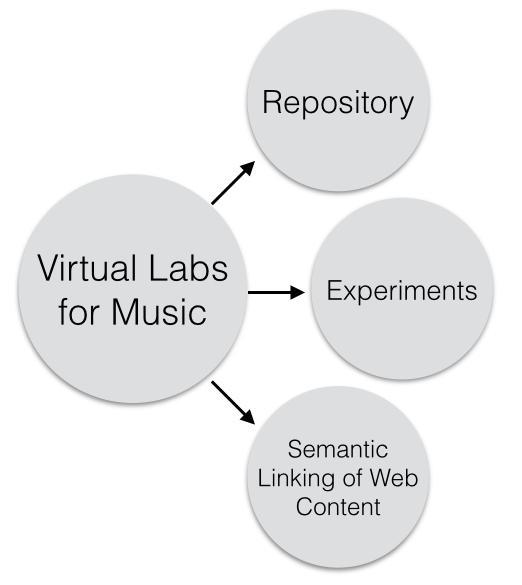
\includegraphics[width=\linewidth]{fig1.png}
  \caption{Sections in the Virtual Labs}
  \label{fig:marginfig}
\end{marginfigure}

\subsection{Changing Modes of Pedagogy in HCM}\label{sec:pedagogy}
Hindustani Music traditionally evolved as an art form requiring years and years of guided practise. In ancient times, students of classical music would spend several years with their teachers studying under their scrutinized guidance and slowly absorbing the intricate nuances of the musical performance from the guru. \cite{neuman} Artists were often patronized by princely states and kings and taught students in this system called the \textit{gurukul} system. This started to change towards the end of the 19th century when music reform and education were taken up as a cause by several conferences of music and scholarly musicians of the time.\cite{mansions} At the time of reform of Indian universities, musical education paradigms changed drastically and musical education was restructured to fit the bounds of a degree education. This meant that the years that could be spent on slowly cultivating musicality and other skills needed to be condensed in a much shorter span. The pedagogical methods changed and the restructuring of courses around study material was a huge challenge of the times. As the twentieth century progressed, both these modes of learning - the traditional way and also the way of classes and tuitions - grew side by side.

\subsection{Twenty First Century}After several changes in musical education, we now have come to the time when musical content isn't learnt continuously by being around music, but in shorter lessons, which are sometimes conducted with multiple students learning together. Lessons are usually structured to be once in a week, and the students are expected to prepare a lot of material by themselves with un-aided, unaccompanied practise. This means that several critical skills, that earlier were absorbed by students by being around music a lot, are expected to be naturally developed by them either as time passes or through their own practice. This calls for students being able to arrange for their own practise without the presence of other musicians. To support this, several modern electronic instruments have been invented as replacements for accompaniment in the last twenty years, aiding musical practise greatly. Electronic Tanpura, Tabla, Lehra and Shruti box are now commonly seen not just in practise settings but also on the performing stage. Despite this being true, the methods of learning musicological concepts haven't been truly exploited through electronic and computer methods. Having said this, there is no parallel development in music learning applications for students of Hindustani Music. 

\subsection{Notation and Musicianship at odd angles} V N Bhatkhande developed a comprehensive scheme for notation of classical music in the early 1900s. \cite{bhatkhande} His contemporary, V D Paluskar developed a parallel style of notation which is slightly similar to Bhatkhande's. Since then, there have been several notation systems that extend these and bring out more nuances. Bhatkhande's system remains to be the most popular one and is widely used. This has changed musical study greatly. It is now common practise now for students to write the new compositions they have been taught. Composing new structures on paper first is also exceedingly common. However, there haven't been comprehensive and accessible repositories of such music that are available to everyone. Resource books that contain western notations of HCM have also been produced for reference and learning. \cite{kauffman} \cite{ragaguide} Most of this music is written so long ago that it is sung simultaneously in different ways across several \textit{gharanas} and several different composers at the same time, and all of these renditions and years of practise have lent their own modifications to those compositions.\cite{jairazbhoy} New students of music often learn to compose their own music by writing down, in this form of notation, their own drafts of improvisation and so forth. Several scholars dismiss notation and writing down, saying that Hindustani Music is meant to be assimilated and never written down. Despite this insistence, it is important to acknowledge the social changes that have led to a changing lifestyle for musicians and music learners, who devote time and resource towards the study of music a lot differently than what they had been doing.
\paragraph{}Given this background, it is only natural for the development of musicianship to train for these singular skills with drills that are suitable to the constraints of time that they have.

\begin{marginfigure}%
  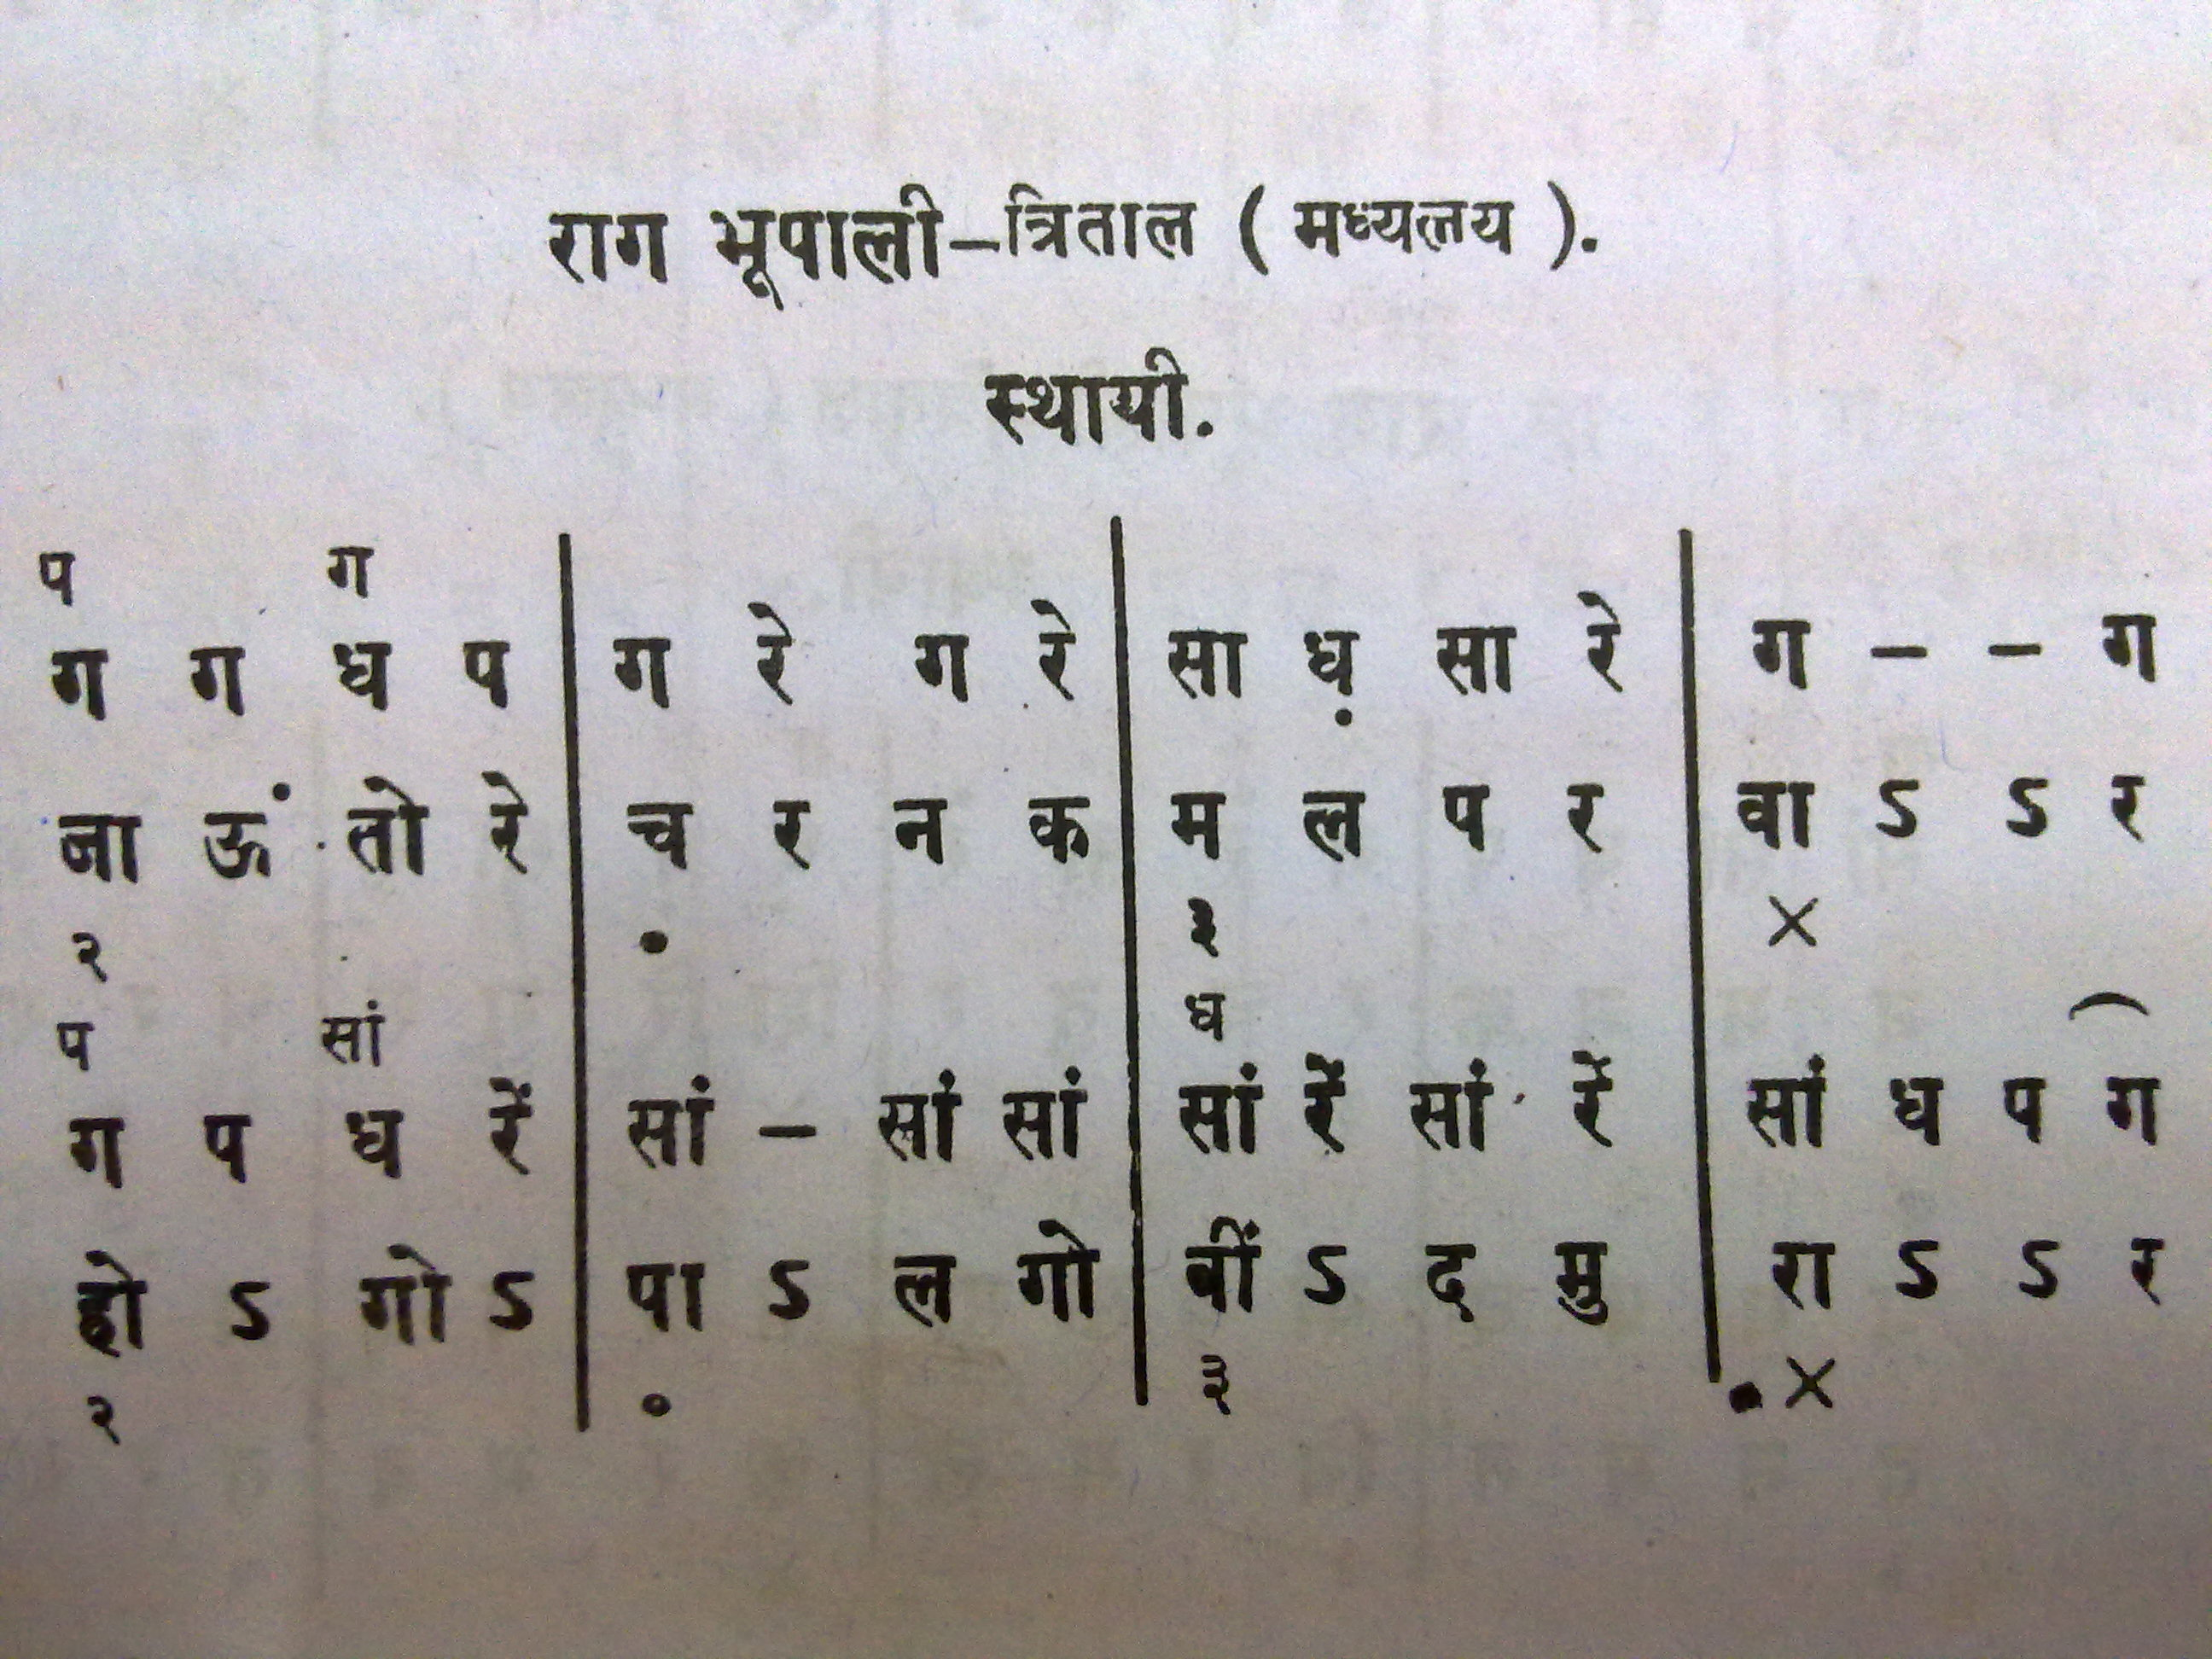
\includegraphics[width=\linewidth]{bhatk1.jpg}
  \caption{Sections in the Virtual Labs}
  \label{fig:marginfig}
\end{marginfigure}
\subsection{On-line Repositories}
\paragraph{Resources for other genres} There is a
great deal of resource material available on the web for
several genres of music, including Western
Classical\cite{IMSLP-petrucci}, Jazz and
Folk\cite{smithsonian}.  These include resources and
websites that help practice ear training skills, or provide
repositories for compositions from different time periods,
databases of lyrics of various arias, right up to
recognising the versions of different compositions and
publications of musical material.  Sadly, this isn't true
for Hindustani music.

\paragraph{Web music resources for Hindustani and Carnatic music}
Currently, the resources on the web for Hindustani music are
scattered and disorganised \cite{sra,ncpa}.  Descriptions of
ragas and performances or performers have been blogged
about\cite{parrikar,deepakraja}.  Youtube videos of
different performances form a sizeable chunk of the material
available for listeners.  The material is often poorly
annotated.  Other sites keep information only available
behind a pay-wall \cite{swarganga}.  There is a need for
organising and inter-linking existing material so that
Hindustani music along with annotations, commentaries and
other related content are made more openly and widely
accessible.  There is also a need to create repositories for
listeners so that they can self-learn to listen to classical
music and appreciate the nuances of this style.
%
\subsection{Cultivation of Musicianship skills} Critical musicianship abilities are a prerequisite for becoming a learned singer in HCM. These include the ability to identify notes and note names from hearing music. A musician is expected to be able to identify and notate rhythm, to be able to work with laya, to be able to be a good presenter and so forth. All proficient performers are expected to be comfortable with these skills, although there is no systematic method to cultivate them. Skills like swara identification and being able to notate and identify musical patterns, although required, is a hard skill to develop on your own. For vocalists who don't play an instrument, for instrumentalists who don't sing or aren't required to notate, this task is challenging. Without guidance, through pure listening, these skills take years to come to grips with \textit{Swar-Jnyan} (Knowledge of pitch). Another area that is typically required and often very hard to develop is the proper knowledge of intonation. Hindustani Music uses microtonal scales, and something as simple as tuning a \textit{Tanpura} requires immense expertise and very finely developed ears. It typically takes students years to master this if they are taught. If they are never taught these skills, which happens many a times in tuition-class like model of teaching Hindustani music, these skills remain undeveloped. This challenge is faced by several new students who study music using new methods such as reading from texts, learning with teachers over the internet and so forth. These abilities need to be developed and taught in new way. 

\subsection{Propositions for Novel Methods to introduce musical material}
We propose a drill-based practice approach towards learning these critical skills of musicality.
Ours is a tripartite approach towards archiving, learning and distribution of classical music. This includes both musicians and non-musicians being able to experiment with music in all capacities. The experiments will enable musicians to be able to engage with experiments to hone their musical skills as well as understand finer and finer nuances of musical listening. 
\paragraph{Power of Drilling} Battery of tests and a system adapting to the ability level of the student is what is needed in such a case, for teaching these specific skills to students. 

\section{Computational and Cognitive Aspects of HCM}
Computational research in musical creation and cognition have become established fields for study of music in pedagogy, therapy and for its cognitive effects. This approach towards the study of music is becoming popular even for Hindustani music, and has tremendous applications for use in pedagogical, and educational contexts. The forms and function of music beyond its aesthetic value, its contribution to other cognitive systems such as visuo-spatial abilities, language learning potential and so on. Systematic studies regarding Hindustani music could become easier after systematizing the methodology for musical categories, and ease in recording and analysing the performance of a general population in different music-related abilities.  
Research work with regards to these various aspects of cognition and computation could be carried out easily through such a lab. Some
examples are: understanding the generation of mood of
\emph{rasa} or \emph{raga} becoming alive, pedagogical
methods to enhance learning and practice, generative
structures of raga and so on and so forth. It would also be
an important task in this project to generate a formal
ontology of Hindustani music which would make it easy to
understand not only the structures of music, but also
meta-tag and retrieve more data from the new musical uploads
that are generated.

\paragraph{Research in pedagogy}
Learning Hindustani music on the internet is a recent phenomenon. With the help of technology, we can enable a student to access guided practice, simulate drilling and give feedback about
intonation, provide analysis for practice etc. There is also
the scope for learning patterns from large data which can be
mapped to student performance for further anlaysis and
feedback. This might help us understand the actual context of musical learning and how it can be best adjusted to help most people learn seamlessly.


\section{Three Fold Approach Structure}

\paragraph{A 3-Fold Approach to Musical Learning} The
objective of this lab would be to provide material in the
following ways:

\begin{enumerate}

\item \textbf{Content Aggregation}

  This would involve creating a repository for notated
  classical music. This would include renotating openly
  available material on classical music, and putting up old
  material that is still used as a reference and sung -
  online. Some of this material could also be
  crowdsourced. Stylistic instruction and para-musical
  features would also be enumerated.

\item \textbf{Experimenting with musical Concepts}

  This section would include experiments that visitors can
  perform to experiment with musical ideas and enhance their
  knowledge and understanding of classical music.


1. Listener perspective \\

The appreciation of any musical genre is greatly enhanced by
understanding. In this section there would be experiments to
increase the understanding of musical form, notes, moods,
and so on. This may be in the form of discrimination tasks,
identification or memory tasks for small musical
samples. The visitors would also be allowed to change some
variables and experiment with the musical form.

2. Student perspective\\

For a student or a prospective performer, it is important to
experiment with different concepts of composition. Creating
a grammatical phrase in a raag, then an aesthetically
pleasing phrase, and then recombination of phrases in an
aesthetic manner - these are some examples of critical
practice that a student has to undergo while studying
music. We will create some experiments to enable users
perform such practice easily through this lab.

\item \textbf{Annotation and re-narration of web content}

  As mentioned above, the current state of the content is in
  the form of youtube videos, annotations on blogs and so
  on. When music is written down in the blogs and talked
  about, it is very hard for an uninitiated listener to
  understand the nuanced language of describing music. Here
  we plan to use a framework for re-narration and annotation
  of musical content from other sources such as links to
  other pages, audio re-narrations, explanations in simpler
  language and so on. This would make the experience of the
  web for music truly multi-modal and rich.

\end{enumerate}

\section{Deliverables}
The following will be the deliverables for this project:
\begin{itemize}

\item Experiment Portal\\
This portal will contain a complete list of experiments in two sections:
\begin{itemize}
\item Music Learning Experiments\\
These experiments will be designed for teaching students of music some elements of musicianship and providing them with drills for learning.
\item Music Appreciation Experiments\\
These experiments will teach the users how to appreciate musical nuances and what to look for in HCM.

\end{itemize}
\item Repository\\
This section will contain resource material for popular khyals in HCM, notated. It will also contain the following:
\begin{itemize}
\item Repository of Khyals
\item Raga-Net: A graph visualization of Concepts, Ragas, Gharanas, Artists and so forth in HCM
\item Links between 
\end{itemize}

\item Behavioral and Cognitive Science Experiments for Music\\
\begin{itemize}
\item Analyzing data from demographic - Musical abilities of music learners 
\item Vocalization and native language - How do vocal habits and articulation of the mother tongue language affect and change the singing voice

\end{itemize}

\item Linked Resources\\

\end{itemize}

\section{Timelines}


\begin{table}[h]
\begin{tabular}{ll}
\toprule
Version 1                    & Contents      \\
\midrule
Experiment Portal              & All Pitch-Related Experiments\\
Repository                     & Database\\
Ontology & Semantic ontology consisting of\\ 
 & raga distances and definitions\\
\bottomrule    
\end{tabular}
\caption{Version 1. Release date: October 30}
\end{table}

\paragraph*{}
After obtaining feedback from the users of this portal, the experiments will be updated

\begin{table}[h]
\begin{tabular}{ll}
\toprule
Version 2                    & Contents      \\
\midrule
Experiment Portal & All Rhythm and Instrument\\ & Experiments\\
Repository & Crowdsourcing khyal documents\\
Ontology & Visualization of Raga Ontology\\
& Queriable ontology create\\
\bottomrule    
\end{tabular}
\caption{Version 2. Release date: January 30}
\end{table}


\begin{table}[h]
\begin{tabular}{ll}
\toprule
Version 3                    & Contents      \\
\midrule
Experiment Portal              & Raga and Khyal relation\\
& related experiments\\
Repository                     & Releasing bandish databases\\
& from collected repositories\\
Ontology & Mapping contemporary compositions\\
 & to ontologies\\
\bottomrule    
\end{tabular}
\caption{Version 3. Release date: March 30}
\end{table}


\begin{table}[h]
\begin{tabular}{ll}
\toprule
Version 4                    & Contents      \\
\midrule
Experiment Portal              & Gamification of All Experiments\\
Repository                     & Provide a searchable database of bandishes\\
 & Collecting private Bandishes from people\\
Ontology & User Privileges to add \\ 
& content from other sources\\
\bottomrule    
\end{tabular}
\caption{Version 4. Release date: May 30}
\end{table}

\section{Budget and Resources }
\label{sec-1}
\subsection{HR}
\label{sec-1-1}


\begin{center}
\begin{tabular}{lrrrl}
\hline
 Item           &   Cost  &       &         &     \\
                &  (L/y)  &  No.  &  Total  &     \\
\hline
 MS Student     &    3.5  &    1  &    3.5  &     \\
\hline
 Engineer       &    4.5  &    1  &    4.5  &     \\
\hline
 Research Asst  &    1.5  &    1  &    1.5  &     \\
 (S/W)          &         &       &         &     \\
\hline
 Total          &         &       &    9.5  &     \\
\hline
\end{tabular}
\end{center}
\subsection{Equipment}
\label{sec-1-2}



\begin{center}
\begin{tabular}{lrlll}
\hline
 Equipment       &        &     &     &     \\
\hline
 Field Recorder  &   .20  &     &     &     \\
\hline
 Mic             &  0.05  &     &     &     \\
\hline
 Mixer           &  0.15  &     &     &     \\
\hline
 Mac Laptop      &  0.80  &     &     &     \\
\hline
 Total           &   1.2  &     &     &     \\
\hline
\end{tabular}
\end{center}
\subsection{Consumables}
\label{sec-1-3}



\begin{center}
\begin{tabular}{lrlll}
\hline
 Server hosting  &  0.20  &     &     &     \\
\hline
\end{tabular}
\end{center}
\subsection{Travel}
\label{sec-1-4}



\begin{center}
\begin{tabular}{lrlll}
\hline
 Visits to            &       &     &     &     \\
 Music Colleges       &    1  &     &     &     \\
 and Museums          &       &     &     &     \\
\hline
 National Conference  &  0.5  &     &     &     \\
\hline
 International        &    3  &     &     &     \\
 Conference           &       &     &     &     \\
\hline
 Total                &  4.5  &     &     &     \\
\hline
\end{tabular}
\end{center}
\subsection{Total}
\label{sec-1-5}



\begin{center}
\begin{tabular}{lrlll}
\hline
                    &    9.5  &     &     &     \\
\hline
                    &    1.2  &     &     &     \\
\hline
                    &    0.2  &     &     &     \\
\hline
                    &    4.5  &     &     &     \\
\hline
 Total              &   15.4  &     &     &     \\
\hline
 @0.15 contingency  &   2.31  &     &     &     \\
\hline
 Total              &  17.71  &     &     &     \\
\hline
\end{tabular}
\end{center}

\section{Conclusions}
There is thus an immense potential to channel the information in Hindustani music into a computer based resource for education, deepening cognitive understanding of music, as well as developing web architecture that supports the multimodal requirements of musical material.

The lab will support drills in musicianship, fitting into the ever changing pedagogical practises of Hindustani Music. A repository that will also enable computational experiments in extending the bounds of experimentation in Hindustani Classical Music. 

This will be the broadest attempt of its kind to fit the missing pieces together, and will serve as a massive source of information.

\bibliography{sample-handout}
\bibliographystyle{plainnat}

\section{Appendix - Description of Some Concepts Mentioned}

\subsection{Sample Set of Experiments}
\paragraph{Expt 1 Pitch discrimination}
This experiment will focus on students being able to distinguish
between two pitches that are played consecutively. The students will
only to answer whether the two pitches played are the same or
different.
\paragraph{Expt 2 Pitch Direction}

This subsequent experiment focuses on being able to identify the
direction of difference of the given pitches. After the student is
comfortable telling two tones apart, this experiment will help them
understand whether the subsequent tone is lower or higher than the
first.
\paragraph{Expt 2.5 What are notes?}
This experiment will explain the concept of notes and
octaves. Students will learn to identify octaves and figure out how
notes played in a row sound. Different instruments can be used to
elaborate this. For vocalists, this may include clicking on the names
of svaras / intervals and then listening to them. Students will also
be able to play notes as scales with note names to familiarize with
the concept of naming notes.\\
Before we move to interval identification, this experiment is a free
exploration of musical hearing.

\begin{itemize}
\item 1. Free exploration with instrument and note names

\item 2. Free exploration hearing different scales and note sequences\\
\end{itemize} % ends low level

\paragraph{Expt 3 Pitch identification from same tonic}

Here we start to move to interval hearing and tone training. \\
Before being able to train the ear for identifying pitches, this
simple experiment will help students distinguish between 

\begin{enumerate}
\item Levels
\begin{enumerate}
\item Level 1: Sa, Ma, Pa
\item Level 2: + Ga, Ni
\item Level 3: + Re, Dha
\item Level 4: All Shuddha Notes
\item Level 5: + Re Dha Komal
\item Level 6: + Ga Ni Komal
\item Level 7: + Tivra Ma
\item Level 8: All notes
\end{enumerate}
\item Number of Questions
\end{enumerate}

\paragraph{Expt 4 Pitch identification from separate tonic}
While the tanpura is playing in another key, a different reference
note will be given to judge another pitch interval from.\\
This experiment is to build hearing independence outside the tonic, as may be required in some forms of light classical singing.
\paragraph{Expt 5 Identifying a chain of pitches}
In this experiment, the experimenter will have to name the notes in a row of pitches in a single tonic. This experiment will decelop the knowledge of `svar-sthan' in the users.
\begin{enumerate}
\item Levels
\item Number of Questions per level
\end{enumerate}
     
\paragraph{6 Tabla Simulation}
The goal of this experiment is to simulate a tabla skin on a computer,
and choose and handshape, and simulate the sounds that a tabla makes
if it is struck at different points.\\ 
Understanding tabla bols also requires an understanding of how it is
played on the skin membrane. This experiment will help people who
don't have access to tablas to explore the instrument in detail.

\begin{enumerate}
\item Hearing bol and location of playing
\item Composing new taals
\end{enumerate}
     
\paragraph{Expt 7 Khali and Taali}
This experiment is to explain the polarity between these two events in
Taal. The rhythmic and motional feeling of a downbeat and an upbeat
will be explained. Participants will get to freely explore and listen
to tabla sounds, and figure out the presence of khali and tali in the taals.
\begin{enumerate}
\item Analyzing khali and taali in visual form
\item Building larger metrical structures for khali and tali
\item Splitting These structures into different laya combinations - aad, kuaad, bayaad
\end{enumerate}
\paragraph{8 Singing and melograph plotting}

Dynamic capture of musical voice and generation of melographs dynamically with 

Melographs are a visual representation of the sung music. This
experiment will help people familiarize themselves with a visual
scheme to understand music. This scheme will be taken forwards

\begin{enumerate}
\item Matching own melograph with template melographs
\item Difference measure for melographs
\end{enumerate}


\subsection{Sample Research Questions}

\begin{itemize}
\item Musical Proficiency in General Population\\
There are no real numbers to determine the musical profeciency of a general population. Often, the tests undertaken fail to get contextualized to an ethno-cultural demographic. This portal will enable us to create a space to easily experiment with the data on musical proficiency through the tests built on it.

\item Pedagogical Research on Repetitive Learning\\
What is the best method of teaching somebody to listen to nuances of music? Through this portal, we can try various styles of teaching and see how they perform on an average for a general population.

\item Musical Absorption and Rasa Theory\\
Experiments can be built to check the involvement of musical listeners and musicians in the emotional content as described in the Rasa theory, and to better map it to ragas, raga times and so on.
\end{itemize}
\end{document}
